\documentclass[conference]{IEEEtran}
\IEEEoverridecommandlockouts

\usepackage{amsmath,amssymb,amsfonts}
\usepackage{algorithmic}
\usepackage{graphicx}
\usepackage{textcomp}
\usepackage{xcolor}
\usepackage{biblatex}
\usepackage{comment}
\addbibresource{refs.bib}

\def\BibTeX{{\rm B\kern-.05em{\sc i\kern-.025em b}\kern-.08em
    T\kern-.1667em\lower.7ex\hbox{E}\kern-.125emX}}
    
\begin{document}

\title{BPC-PRP Project}

\author{\IEEEauthorblockN{1\textsuperscript{st} Jan Němec}
\IEEEauthorblockA{\textit{BPC-PRP} \\
\textit{VUT} \\
{Brno, Česká republika \\
247432}} 
\and
\IEEEauthorblockN{2\textsuperscript{nd} Erik Scholz}
\IEEEauthorblockA{\textit{BPC-PRP} \\
\textit{VUT} \\
Brno, Česká republika \\
247462}
}
\cr
\maketitle

\begin{abstract}
Práce se zabývá popisem řešení závěrečného projektu pro předmět BPC-PRP na VUT. V první části jsou vysvětleny podmínky a cíle útěku z bludiště. V druhé části je stručně popsán robot, s kterým byl projekt splněn a je zde popsán návrh a řešení projektu, jako je průjezd koridorem, otáčení na konci koridoru, průjezd křižovatkou a čtení aruco tagů pro efektivní průjezd bludištěm.
\end{abstract}

\begin{IEEEkeywords}
Robotics, project, BPC-PRP, state-of-the-art
\end{IEEEkeywords}


\section{Úvod}





Navigace autonomních robotů v neznámém prostředí je jedním z klíčových problémů řešených v oblasti robotiky. Efektivní orientace v prostoru bez předchozí znalosti prostředí je zásadní u průzkumných nebo záchranných misí.

Cílem tohoto projektu bylo navrhnout a implementovat algoritmus řízení univerzitou poskytnutého robota tak, aby byl schopen samostatně projít celým bludištěm za co nejrychlejší čas bez jakéhokoliv dotyku nebo kolizí se stěnou bludiště.

Bludiště bylo sestaveno jako nepravidelná síť chodeb sestavená z buněk o rozměrech 40x40 cm a ven vedla pouze jedna trasa. Nacházely se zde i slepé uličky, penalizace ve formě "setkání s Minotaurem" a časový bonus při nalezení pokladu. Na zemi byly umístěny aruco tagy, které určovaly nejkratší únikovou trasu z bludiště na křižovatkách.

Cílem této práce je popsat návrh implementaci a výsledky námi navrženého algoritmu řízení robota v diskrétním prostoru, který mu umožnil utéct z bludiště.

\section{Řešení a popis}
\subsection{Popis robotu}

Robot, se kterým jsme v rámci úlohy pracovali, je mobilní platforma vybavena širokou škálou senzorů potřebných pro autonomní navigaci v bludišti. Robot je sestaven ze tří pater, každé vybavené jinými senzory a hardwarem pro různé účely.

Základní spodní patro této platformy je tvořeno diferenciálním dvoukolovým podvozkem, který umožňuje nezávislé řízení levého a pravého kola. Díky umístění kol uprostřed konstrukce je robot schopen otáčet se dokola na místě, což je pro navigaci v diskrétním prostoru bludiště obzvlášť výhodné. Motory jsou také vybaveny inkrementálními čítači, díky kterým lze měřit otáčky motoru a nebo je využít k odometrii. Nalezneme zde také dva senzory umístěné na přední straně robotu, které jsme v  dřívější úloze využili k pohybu robota po čáře.

Druhé patro robota obsahuje většinu senzorů, které umožňují vnímání okolního prostředí a kvalitní orientaci autonomního systému. Hlavním senzorem je zde 360° Lidar, který je umístěn uprostřed robotu. Díky tomuto senzoru je systém schopný zjistit svoji vzdálenost od stěn bludiště. Dalším senzorem, který zde nalezneme, je trojice ultrazvukových senzorů. Senzory jsou umístěny na přední straně robotu, jeden uprostřed přední stěny směřující dopředu a dva ostatní symetricky umístěny po stranách pod lehkým úhlem. Tuto trojici snímačů lze využít k detekci stěny a zabránění nárazu. Nalezneme zde i držáky na dvě 10000 mAH baterie, jedna z nich určená k napájení podvozku, druhá k napájení dvou horních pater. Posledním senzorem na tomto patře je IMU jednotka, díky které je robot schopen měřit jeho zrychlení a úhlovou rychlost, kterou následně může využít například při otáčení v zatáčkách koridoru.

Na třetím patře se nachází samotný řídící systém robotu, o který se stará Raspberry Pi spolu se zpracováváním získaných dat ze senzorů. Nalezneme zde také jednoduché uživatelské rozhraní s tlačítky a displejem. Nachází se zde také poslední senzor, a to RGB kamera směřující pod úhlem k zemi. Díky tomu je schopna snímat ArUco tagy umístěné v bludišti a následovat optimální únikovou trasu.

Celková konstrukce robota je modulární, což usnadňuje přístup k jednotlivým komponentům a umožňuje jednoduchou údržbu nebo budoucí rozšíření.






\subsection{Popis řešení}
\begin{comment}
\begin{figure}[h]
    \centering
    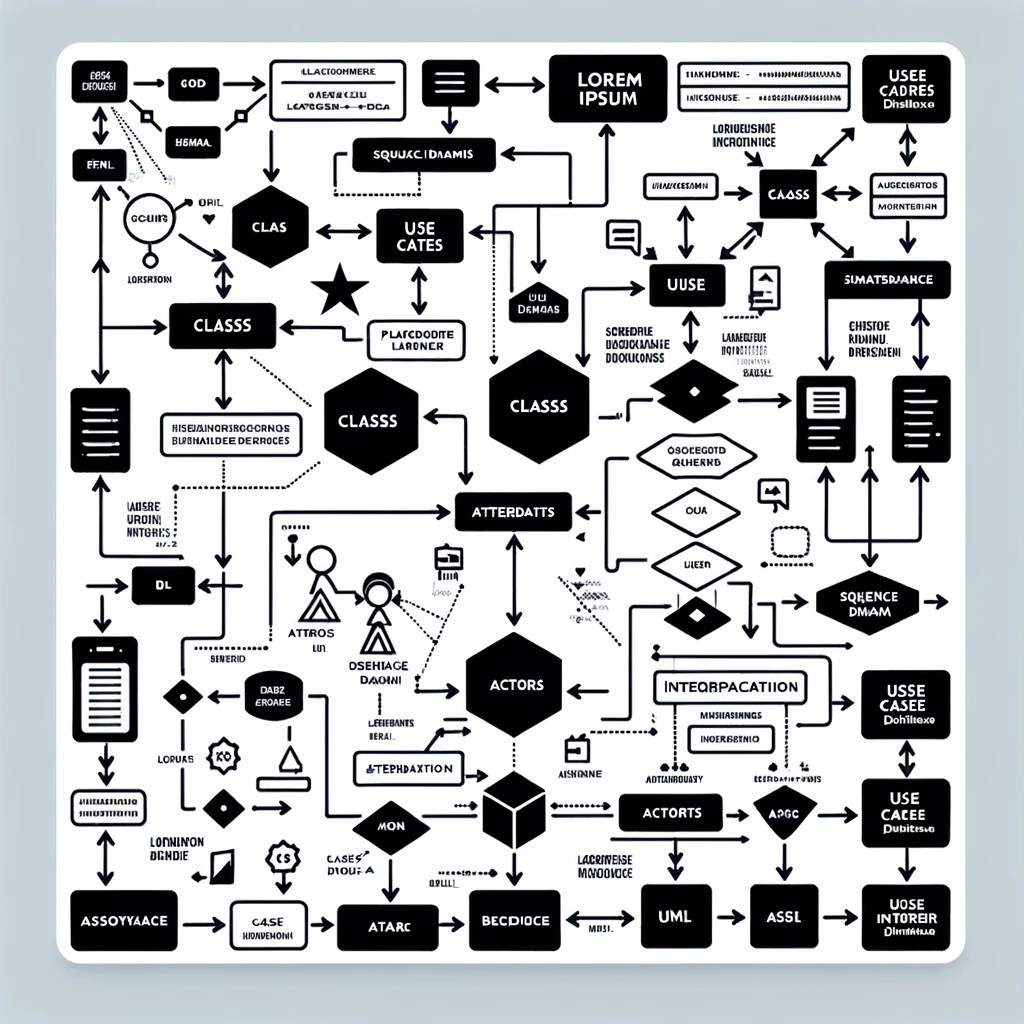
\includegraphics[width=0.45\textwidth]{images/schema.jpg}
    \caption{The schematic}
    \label{fig:schema}
\end{figure}
\end{comment}

\begin{comment}
Robot s kterým jsme pracovali má diferenciální dvoukolový podvozek. Disponuje různými senzory. Pro měření vzdálenosti je vybaven Lidarem schopným měřit v rozsahu 360° a třemi ultrazvukovými senzory. Pomocí enkoderů je schopný měřit otáčky jednotlivých kol. Pro natáčení má zabudován IMU. Dále je vybaven RGB kamerou a Line senzory.

Napájen je z dvou 10000 mAH baterií. O vykonání softwaru se stará Raspberry Pi a Arduino
\end{comment}

\begin{comment}
\begin{figure}[h]
    \centering
    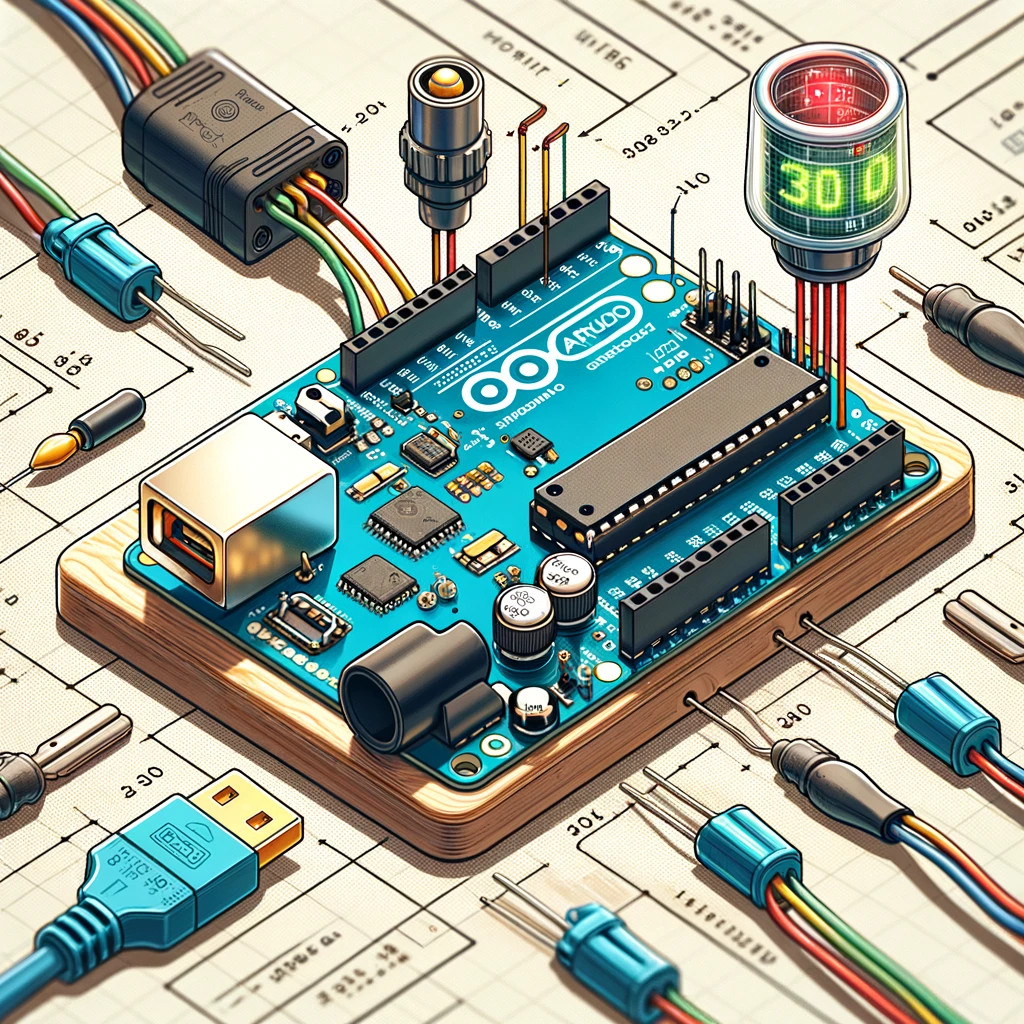
\includegraphics[width=0.45\textwidth]{images/arduino.jpg}
    \caption{Arduino}
    \label{fig:arduino}
\end{figure}
\end{comment}

Řešení můžeme rozdělit na několik dílčích částí: výběr módu, průjezd koridorem, zatáčení v koridoru, čtení ArUco tagů, detekce křižovatek a rozhodování na křižovatkách.

Při spuštění robotu je nejprve zapotřebí stiskem jednoho ze tří tlačítek vybrat mód, ve kterém následně bude robot operovat. Jmenovitě to jsou módy: LINE FOLLOWING, CORRIDOR FOLLOWING a MAZE ESCAPE. V rámci této práce se zaměříme výhradně na třetí režim, tedy MAZE ESCAPE, který byl navržen k samostatné orientaci robota v bludišti a umožnil mu utéct.

Průjezd bludištěm je řízen pomocí stavového automatu o třech stavech, kde každý stav řeší konkrétní fázi pohybu. Tyto stavy jsme definovali jako MOVING, DECIDING a TURNING. Výchozím stavem je stav MOVING, ve kterém se robot pohybuje v bludišti. Stav DECIDING slouží k výběru následující a co nejoptimálnější trasy. Poslední stav TURNING se stará o otáčení na křižovatkách nebo zatáčkách v bludišti.

Základem bylo řešení průjezdu buněk bez křižovatek. Při průjezdu koridorem bludiště robot získává data o jeho vzdálenosti od okolních stěn z Lidaru. Náš algoritmus vybírá pouze měření z určitých úhlových rozsahů (vpřed, vzad, vlevo, vpravo), ty následně průměruje a vrací vzdálenosti od překážek ve všech stranách.

Pro udržení ve středu koridoru si robot počítá rozdíl vzdáleností stěn po levé a pravé straně. Pomocí tohoto rozdílu je přes PID regulátor vypočítán akční zásah, který je následně poslán motory kol tak, aby robot se co nejblíže držel středu koridoru. Pokud kterákoliv postranní stěna chybí, nebo je vzdálená více než polovina šířky buňky (tedy 20 cm), algoritmus nastaví změřenou vzdálenost na této straně na 20 cm, čímž vytváří jakýsi virtuální koridor.

Robot se pohybuje rovně konstantní rychlostí, dokud není nedetekována překážka ve vzdálenosti 30 cm před robotem. Po detekci zpomalí, aby se mohl lépe zarovnat se středem buňky a pokračuje k překážce (stěně) do vzdálenosti 20 cm. Zároveň se tím vyřešil i problém, kdy za určitých podmínek data ze senzorů přicházejí pomalu a robot může narazit do stěny. Tímto způsobem mu dáváme o trochu více času, aby mohl včas zareagovat.

Při detekci stěny před robotem ve vzdálenosti 20 cm přejde do stavu DECIDING. Zde se rozhodne podle toho, zda je na křižovatce, nebo pouze v zatáčce. Tato detekce probíhá výpočtem možných následujících tras pomocí údajů o vzdálenosti od stěn. Jako validní cesta se počítá směr, ve kterém je vzdálenost ke stěně větší než šířka buňky (více než 40 cm). Pokud je počet možných cest pouze jedna, nachází se v zatáčce. Dále pokračuje buď vlevo, nebo vpravo podle toho, kde je vzdálenost ke stěně větší (tedy kde má víc místa). Následně se nastaví do stavu TURNING, který se stará o otáčení robotu.

Křižovatky jsou také detekovány za pohybu koridorem, kdy robot periodicky kontroluje, zda se nachází na křižovatce podle způsobu popsaného výše. Pokud je detekována křižovatka, robot dále měří vzdálenost ke stěně před robotem a vypočítává z ní relativní polohu v buňce. Pokud je tato vzdálenost v určitém tolerančním rozsahu okolo středu buňky, robot zastaví a musí se rozhodnout, kam pokračovat dál.

K následování optimální únikové trasy je za chodu programu vytvořená fronta správných odboček, kterou si robot vytváří skenováním ArUco tagů při pohybu v bludišti. Při detekci tagu je zapsáno jeho id určující směr na další odbočce do fronty. Na křižovatce se robot nejprve podívá, zda má ve frontě načtenou informaci o dalším směru. Pokud ano, nastaví rychlost motorů tak, aby se otočil daným směrem. Pokud informaci nemá, rozhoduje se stejně, jako by byl v zatáčce. Po průjezdu křižovatkou označí poslední směr za provedený a na další křižovatce použije k rozhodnutí následující směr ve frontě.

Otáčení ve stavu TURNING jsme řešili pomocí časovače. Předem byly definovány rychlosti otáčení poslané do motorů a také čas, po který se má robot otáčet, aby se vždy otočil kolem své osy o 90 °. Tyto hodnoty jsme experimentálně změřili a nastavili v programu. Tuto metodu jsme zvolili, protože při použití IMU se časem znepřesňují její výsledky a je potřebná delší kalibrace. Pomocí časovače jsme byli schopni dosáhnout velmi rychlého otáčení o 90°. Po vypršení časovače se motory zastavili a stavový automat byl opět přepnut do stavu MOVING. 

\section{Závěr}

Naše řešení se ukázalo poměrně kvalitním, kdy jsme bludištěm projeli zhruba za minutu a čtvrt po odečtení 30 s za poklad. Během řešení jsme narazili na několik problémů, které jsme museli vyřešit. Občas jsme měli problém přečíst ArucoTagy, nejspíš protože při rychlém otáčení se robot nestíhal vrátit na střed koridoru. Proto bylo zapotřebí rychlejší a agresivnější PID regulátor, který by zřejmě stále mohl být lepší. S tímto problémem jsme si vypomohli i přejitím při otáčení na časovač místo IMU. Je to sice méně robustní řešení a pokud bychom chtěli změnit rychlost otáčení, museli bychom experimentálně určit dobu otáčení, ale pro tento úkol nám výrazně zrychlilo čas.
Další problém jsme měli s příchodem dat ze senzorů. Občas nám chvíli nepřicházeli data a tudíž se robot opět vychyloval ze středu koridoru, nebo zavčas nedetekoval stěnu před sebou. Tuto chybu jsme nemohli odstranit, protože byla zřejmě způsobena sítí, ale alespoň jsme při přiblížení ke stěně přední stranou robota, lehce snížili rychlost, aby měl více času než má úplně zastavit.
\begin{comment}
\begin{figure}[h]
    \centering
    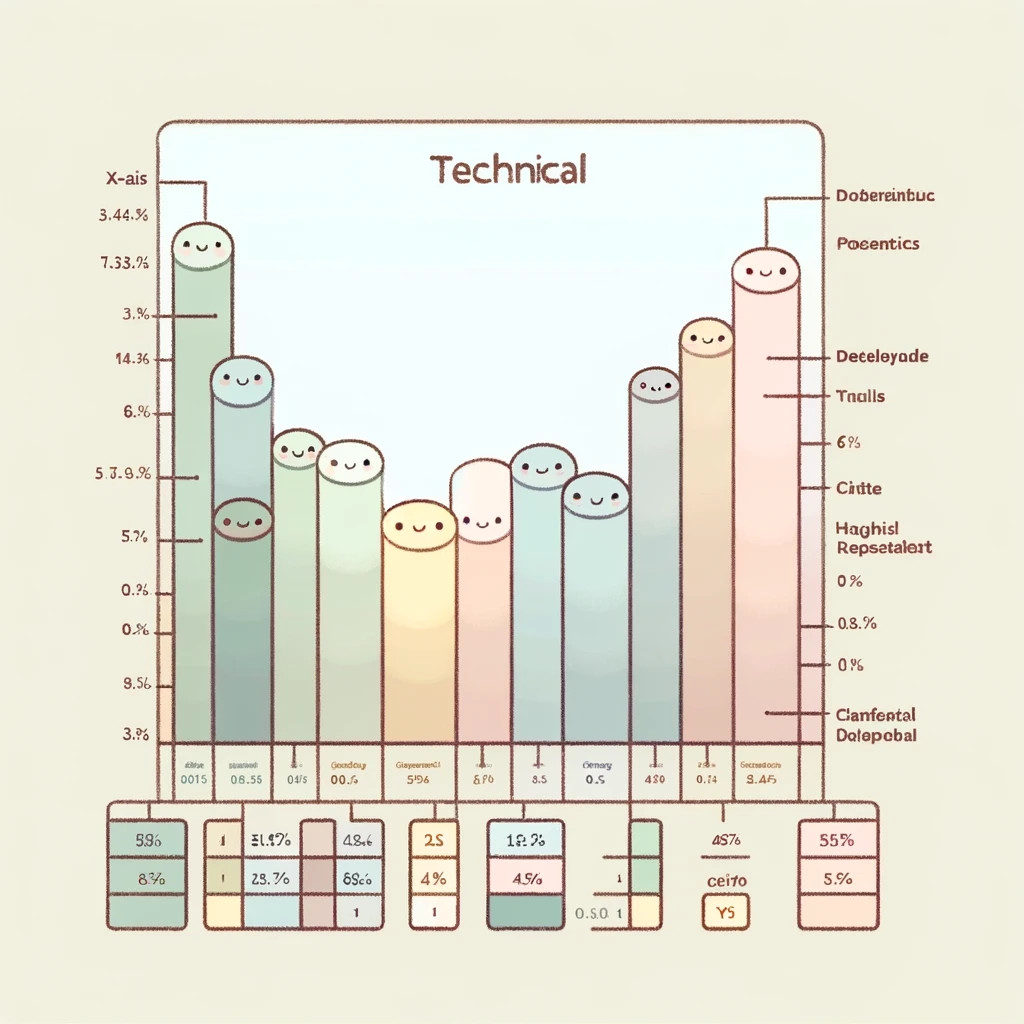
\includegraphics[width=0.45\textwidth]{images/plot.jpg}
    \caption{Plot}
    \label{fig:plot}
\end{figure}
\end{comment}


\section*{Poděkování}
Chtěli bychom poděkovat všem vyučujícím za čas a úsilí věnované během celého semestru. Všichni vyučující byli velmi ochotni pomoci, pokud jsme narazili na problém, nebo jsme si s něčím nevěděli rady. Rádi bychom poděkovali i za samotnou formu vyučování předmětu, která byla velmi zajímavá a zároveň i naučná.

\printbibliography

\end{document}
